\subsection{Generic APIs vs Consumer Driven APIs}

The big decision in micro-frontend API development is to use either generic or consumer-oriented APIs. The difference is that generic APIs place great emphasis on reusability, while consumer-oriented APIs tailor the APIs to the customer.

\subsubsection{Generic APIs}

Generic APIs refer to APIs that are very general and can be used by different clients. However, this type of API has two major drawbacks. Over-fetching describes the problem of getting more data than is needed. Over-requesting describes the problem of needing multiple requests to get the data for a use case. Both problems are discussed in more detail in the next paragraphs. \cite{misc:2019:leitner:background:micro-frontends:backend-for-frontends}

\paragraph{Over-Fetching}

For example, a contact service provides a contact-model that includes customer-number, first-name, second-name, uid-number and the address of the user, as seen in listing \ref{code:state-art:over-fetching}. However, one requirement of the application is to display only a contact's first and last name inside the header. Only two fields of the model are used, and the rest are unnecessarily queried. \cite{misc:2019:leitner:background:micro-frontends:backend-for-frontends}

\ifshowListings
\begin{listing}[H]
    \begin{minted}{typescript}
interface ContactModel {
  id: string;
  customerNumber: string;
  firstName: string;
  secondName: string;
  uidNumber: string;

  Address: {
    id: string;
    postalCode: string;
    location: string;
    Country: string;
  }
}
    \end{minted}
    \caption{Contact-Model that contains too much fields for the requirement.}\label{code:state-art:over-fetching}
\end{listing}
\fi

\paragraph{Over-Requesting}

Attempting to solve the problem of over-fetching by reducing the amount of data set that is returned leads directly to this problem. Listing \ref{code:state-art:over-requesting} shows the problem of over-requesting. If another requirement inside the application should display the address alongside the contact, two requests have to be performed every time. Afterwards, the two data sets have to be merged, which leads to high complexity on the client side. \cite{misc:2019:leitner:background:micro-frontends:backend-for-frontends}

\ifshowListings
\begin{listing}[H]
    \begin{minted}{typescript}
interface ContactModel {
  id: string;
  customerNumber: string;
  firstName: string;
  secondName: string;
  uidNumber: string;

  address_id: string;
}
    \end{minted}
    \caption{Contact-Model model that links the address-model with an id.}\label{code:state-art:over-requesting}
\end{listing}
\fi

\subsubsection{Consumer Driven APIs}

Consumer-driven APIs are the opposite of generic APIs. They follow the idea of providing the client with exactly the data it needs. Following the example above, the contact service would have an endpoint that returns only the first and last name as required for the request. These endpoints make communication with a client very simple and there is not the problem of over-fetching and over-requesting. However, creating an endpoint for each request creates an unmanageable set of endpoints. \cite{misc:2019:leitner:background:micro-frontends:backend-for-frontends}

\bigskip

\noindent To solve these problems, the backend-for-frontend pattern is often used. This pattern provides each client with its own API, which specialized for the needs of the client. \cite{book:2018:richardson:background:bff:microservices-patterns}

\ifshowImages
\begin{figure}[H]
    \centering
    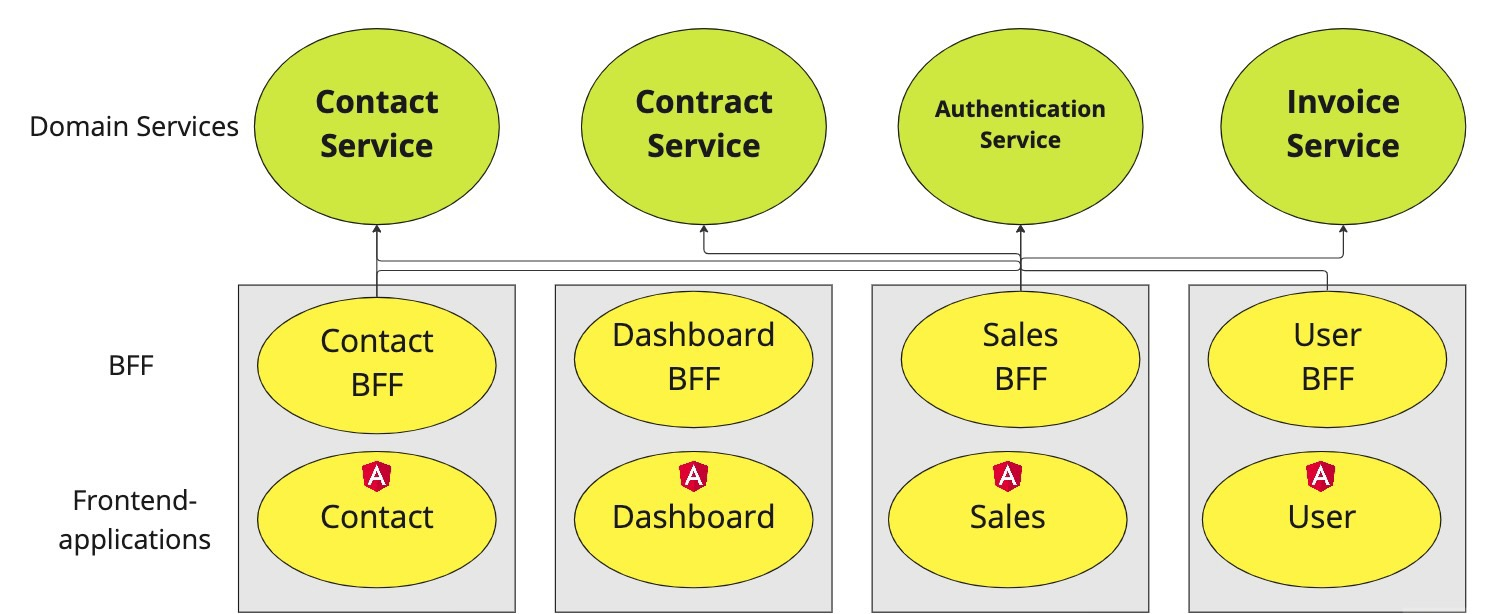
\includegraphics[width=0.8\linewidth]{images/ui-bff-architecture.jpeg}
    \caption{Frontend architecture with the backend-for-frontend pattern.}\label{figure:state-of-the-art:ui-bff-architecture}
\end{figure}
\fi

\noindent Figure \ref{figure:state-of-the-art:ui-bff-architecture} shows an exemplary micro-frontend architecture using the backend-for-frontend pattern. Each frontend has a service that retrieves data only for that specific client. Because the backend-for-frontends function as gateway to the domain services, the domain services can stay very generic and be reused by different clients. Backend-for-frontends should implement only the presentation logic that puts the data into the form that the client needs. It should avoid storing state. \cite{misc:2019:leitner:background:micro-frontends:backend-for-frontends}

\bigskip

\noindent With this architectural approach the backend-for-frontend and the frontend form a single deployment unit. If one application is changed, the other needs needs to adapt the changes. GraphQL is a perfect technology for implementing a backend-for-frontend, because it is specifically designed for implementing the presentation-layer.
